% Just notes
%\documentclass[notes=only]{beamer}

% Both slides and notes
\documentclass[notes]{beamer}

% Just slides
% \documentclass{beamer}

\usetheme{default}

% Used to do math and such (I think...)
\usepackage{amsmath}
\usepackage{amssymb}

% Used to color text (for todos)
\usepackage{xcolor}

\usepackage{algorithm}
\usepackage{algpseudocode}

\usepackage{array}

% Used to embed pdfs from yEd and other sources
\usepackage{graphicx}

% Used to make code listings
\usepackage{listingsutf8}
% Used to adjust the page margin
\usepackage{geometry}
% Used to make code show up in multiple columns to fit more on a printed page.
\usepackage{multicol}

% Used to make tables, figures, etc show up where I want them.
\usepackage{float}

\usepackage{array}

%import figures from photoshop
\usepackage{epstopdf}

% Deal with backwards quotes because evidently Latex doesn't know better.
\usepackage [english]{babel}
\usepackage [autostyle, english = american]{csquotes}
\MakeOuterQuote{"}

% multiple rows
\usepackage{multirow}

% used for lettered bullet points
\usepackage{enumerate}

% http://tex.stackexchange.com/questions/137022/how-to-insert-page-number-in-beamer-navigation-bars
% Add page numbers
\addtobeamertemplate{navigation symbols}{}{%
    \usebeamerfont{footline}%
    \usebeamercolor[fg]{footline}%
    \hspace{1em}%
    \insertframenumber/\inserttotalframenumber
}

\usepackage{mathrsfs}

\newcommand{\TODO}[1]{\textcolor{red}{TODO: #1}}

\newcommand{\argmax}[1]{\underset{#1}{\text{argmax }}}
\newcommand{\cprob}[2]{ \prob{#1 \lvert #2} }
\newcommand{\prob}[1]{\mathbb{P}\left( #1 \right)}
\newcommand{\partialDx}[2]{\frac{\partial #1}{ \partial #2  }}
\newcommand{\inAngle}[1]{\left \langle #1 \right \rangle}


\begin{document}

\title{Deep Learning for Automatic Speech Recognition}
\subtitle{CSCI/LING-5832: Natural Language Processing}
\author{Ryan Hartsfield \and Garrett Lewellen}
\date{April 23, 2015}

\frame{\titlepage}

\begin{frame}
	\frametitle{Outline}
	
	\begin{enumerate}
		\item \textcolor{blue}{Introduction}
		\item Gaussian Mixture Models
		\item Convolutional Neural Networks
		\item Deep Neural Networks
		\item Experimental Results
		\item Conclusions
	\end{enumerate}
\end{frame}
\begin{frame}
	\frametitle{Speech Recognition}
	\begin{center}
		Main goal of any automatic speech recognition system is to take some acoustic signal as input and convert it into a corresponding lexical representation.
	\end{center}
	
	\begin{center}
		Tasks range from very easy to extremely difficult: Number recognition, phone recognition, large vocabulary speech recognition, human-computer, human-human
	\end{center}
	
	\begin{center}
		\textbf{Many variable factors to account for}: environmental noise, speaker variation, vocabulary size, degree of fluency, etc.
	\end{center}
\end{frame}
\begin{frame}
	\frametitle{The ASR Problems}
	\begin{center}
		There are \textbf{four} substantial problems that must be solved in any statistical ASR system:
	\end{center}

	\begin{enumerate}
		\item Acoustic Processing
		\item \textcolor{blue}{Acoustic Modeling}
		\item Language Modeling
		\item The Search Problem
	\end{enumerate}
\end{frame}

\begin{frame}
	\frametitle{Acoustic Processing}
	\begin{center}
		Represent acoustic data in a way that has few model parameters, but maintains necessary linguistic information.
	\end{center}
	\begin{center}
		Main form of feature representation are the mel-frequency cepstral coefficients (MFCCs) extracted from a waveform.
	\end{center}
	
	\begin{itemize}
		\item Convert the spectrum of a window into its cepstrum
		\item Effectively separates the source from filter
		\item Cepstral coefficients are uncorrelated
		\item Use the first 12 (represent the filter), their deltas and delta-deltas for 39 features per frame
	\end{itemize}
	
	\begin{equation*}
		c[n] = \sum_{n=0}^{N-1}\log(|\sum_{n=0}^{N-1}x[n]e^{-j\frac{2\pi}{N}kn}|)e^{j\frac{2\pi}{N}kn}
	\end{equation*}
\end{frame}

\begin{frame}
	\frametitle{Acoustic Modeling}
	\begin{center}
		Given the observation feature vector, estimate an HMM state posterior probability: \begin{equation*}
		\cprob{x}{w}\end{equation*} Where \textit{x} is some acoustic signal as input and \textit{w} is a word, phone, sub-phone, diphone, or triphone. 
	\end{center}
	
	We will explore three ways of estimating this probability:
	\begin{itemize}
		\item Gaussian Mixture Models (GMMs)
		\item Convolutional Neural Networks (CNNs)
		\item Deep Neural Networks (DNNs)
	\end{itemize}
\end{frame}

\begin{frame}
	\frametitle{Language Modeling and Search}
	\begin{center}
		Job of the language model is to estimate the prior probability:
		$\prob{w}$
	\end{center}
	\begin{center}
		This is usually done with an N-gram model like we've seen throughout the semester.
	\end{center}
	\vfill
	\begin{center}
		We normally use GMM-HMM or ANN-HMM hybrids for acoustic/language models. Given these models, we need to find the best sequence of words for the acoustic input.
	\end{center}
	\begin{center}
		Search is normally performed using Viterbi, A* decoding, or N-best.
	\end{center}
	
\end{frame}

\begin{frame}
	\frametitle{Outline}
	
	\begin{enumerate}
		\item Introduction
		\item \textcolor{blue}{Gaussian Mixture Models}
		\item Convolutional Neural Networks
		\item Deep Neural Networks
		\item Experimental Results
		\item Conclusions
	\end{enumerate}
\end{frame}

\begin{frame}
	\frametitle{Gaussian Mixture Models}\TODO{clean up}
	\begin{center}
		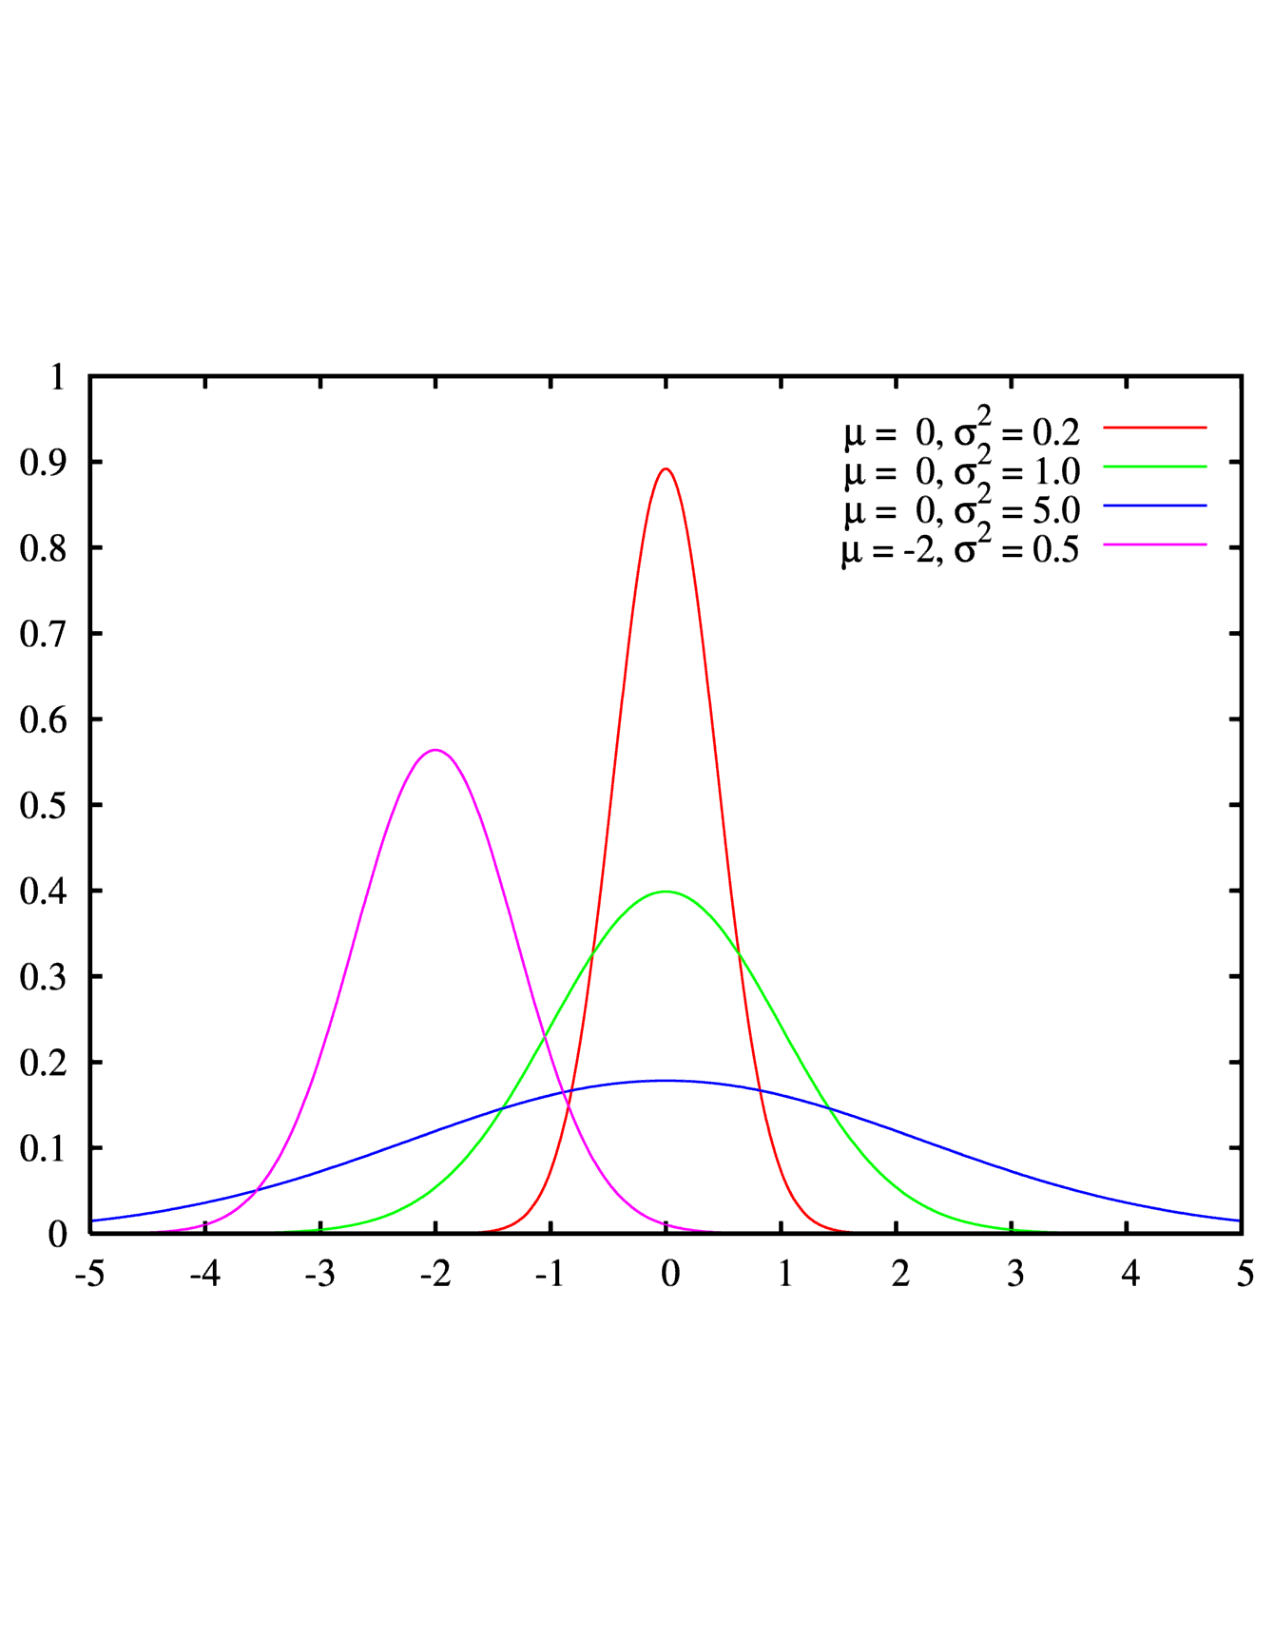
\includegraphics[scale=.3, clip=true, trim=5cm 9cm 4cm 10cm]{gmm.pdf}
	\end{center}

	\begin{center}
		Before the rise of Deep Learning approaches, GMMs were ubiquitous for representing the acoustic model.
	\end{center}
	\begin{center}
		Based on assumption that a mixture of Gaussians can be used to represent the spectral shape.
	\end{center}	

\end{frame}

\begin{frame}
	\frametitle{GMM Models}
	\begin{center}
		Use a weighted mixture of multivariate Gaussians as a model to assign a likelihood to an acoustic observation.
	\end{center}
	
	\begin{center}
	Below is the output likelihood function $b_{j}(o_{t})$:
	\end{center}
	
	\begin{equation*}
	b_{j}(o_{t}) = \sum_{m=1}^{M}c_{jm}\frac{1}{\sqrt{2\pi|\sigma_{jm}|}}\exp[(x-\mu_{jm})^T\sigma_{jm}^{-1}(o_{t}-\mu_{jm})]
	\end{equation*}
	
	\begin{center}
		A GMM model can be trained using the Baum-Welch algorithm to iteratively recompute the mean, mixture weight, and covariance.
	\end{center}

\end{frame}

\begin{frame}
	\frametitle{The Rise of Deep Learning}
	\begin{center}
		Recently, Artificial Neural Networks (ANNs) have experienced great results in a variety of tasks, and ANN-HMMs have begun to replace GMM-HMMs.
	\end{center}
	\begin{itemize}
		\item Increasing processing power and more efficient algorithms for training.
		\item GMMs have much fewer model parameters, and are much easier to train.
		\item ANN-HMM hybrids are much larger, and can take in multiple frames (9-15) 
		\item GMM-HMMs typically only look at a single frame.
	\end{itemize}
	
	\begin{center}
		This increase in size allows hybrid ANN-HMMs to model highly correlated features across wide temporal contexts.
	\end{center}
	
\end{frame}

\begin{frame}
	\frametitle{Outline}
	
	\begin{enumerate}
		\item Introduction
		\item Gaussian Mixture Models
		\item \textcolor{blue}{Convolutional Neural Networks}
		\item Deep Neural Networks
		\item Experimental Results
		\item Conclusions
	\end{enumerate}
\end{frame}

\begin{frame}
	\frametitle{Convolutional Neural Networks}
	\begin{center}
		\textbf{Convolutional Neural Networks for Speech Recognition}
	\end{center}
	
	\vfill
	
	\hfill Ossama Abdel-Hamid \hfill Abdel-rahman Mohamed \hfill Hui Jiang 
	
	\hfill Li Deng \hfill Gerald Penn \hfill Dong Yu \hfill
	
	\vfill
	
	\begin{center}
		IEEE/ACM Transactions on Audio, Speech, and Language processing, Vol. 22, No. 10, October 2014
	\end{center}
\end{frame}

\begin{frame}
	\frametitle{CNN Background}
	\begin{center}
		CNNs have achieved high levels of success in image recognition tasks. They have a very complex architecture that is influenced by our own visual cortex.
	\end{center}
		\begin{itemize}
			\item Special layer with a convolution ply and pooling ply (simple cells and complex cells)
			\item Weights are shared across all neurons in the same convolution ply
			\item Replicates features across the image in order to recognize patterns anywhere within it
		\end{itemize}
\end{frame}
\begin{frame}
	\frametitle{CNN-HMM for ASR}
	\begin{center}
		Apply a similar architecture to the task of ASR with some differences to help exhibit invariance to small perturbations in frequency caused by different speakers, emotional status, background noise, etc.:
		\vfill
		\begin{itemize}
			\item Local Connectivity: Mel-frequency spectral coefficients (MFSC) features
			\item Convolutions along frequency axis: HMMs handle time axis, allow for small frequency shifts
			\item Limited weight sharing: Same pool = Same weights
		\end{itemize}
	\end{center}
\end{frame}

\begin{frame}
	\frametitle{Input Structure of the CNN}
	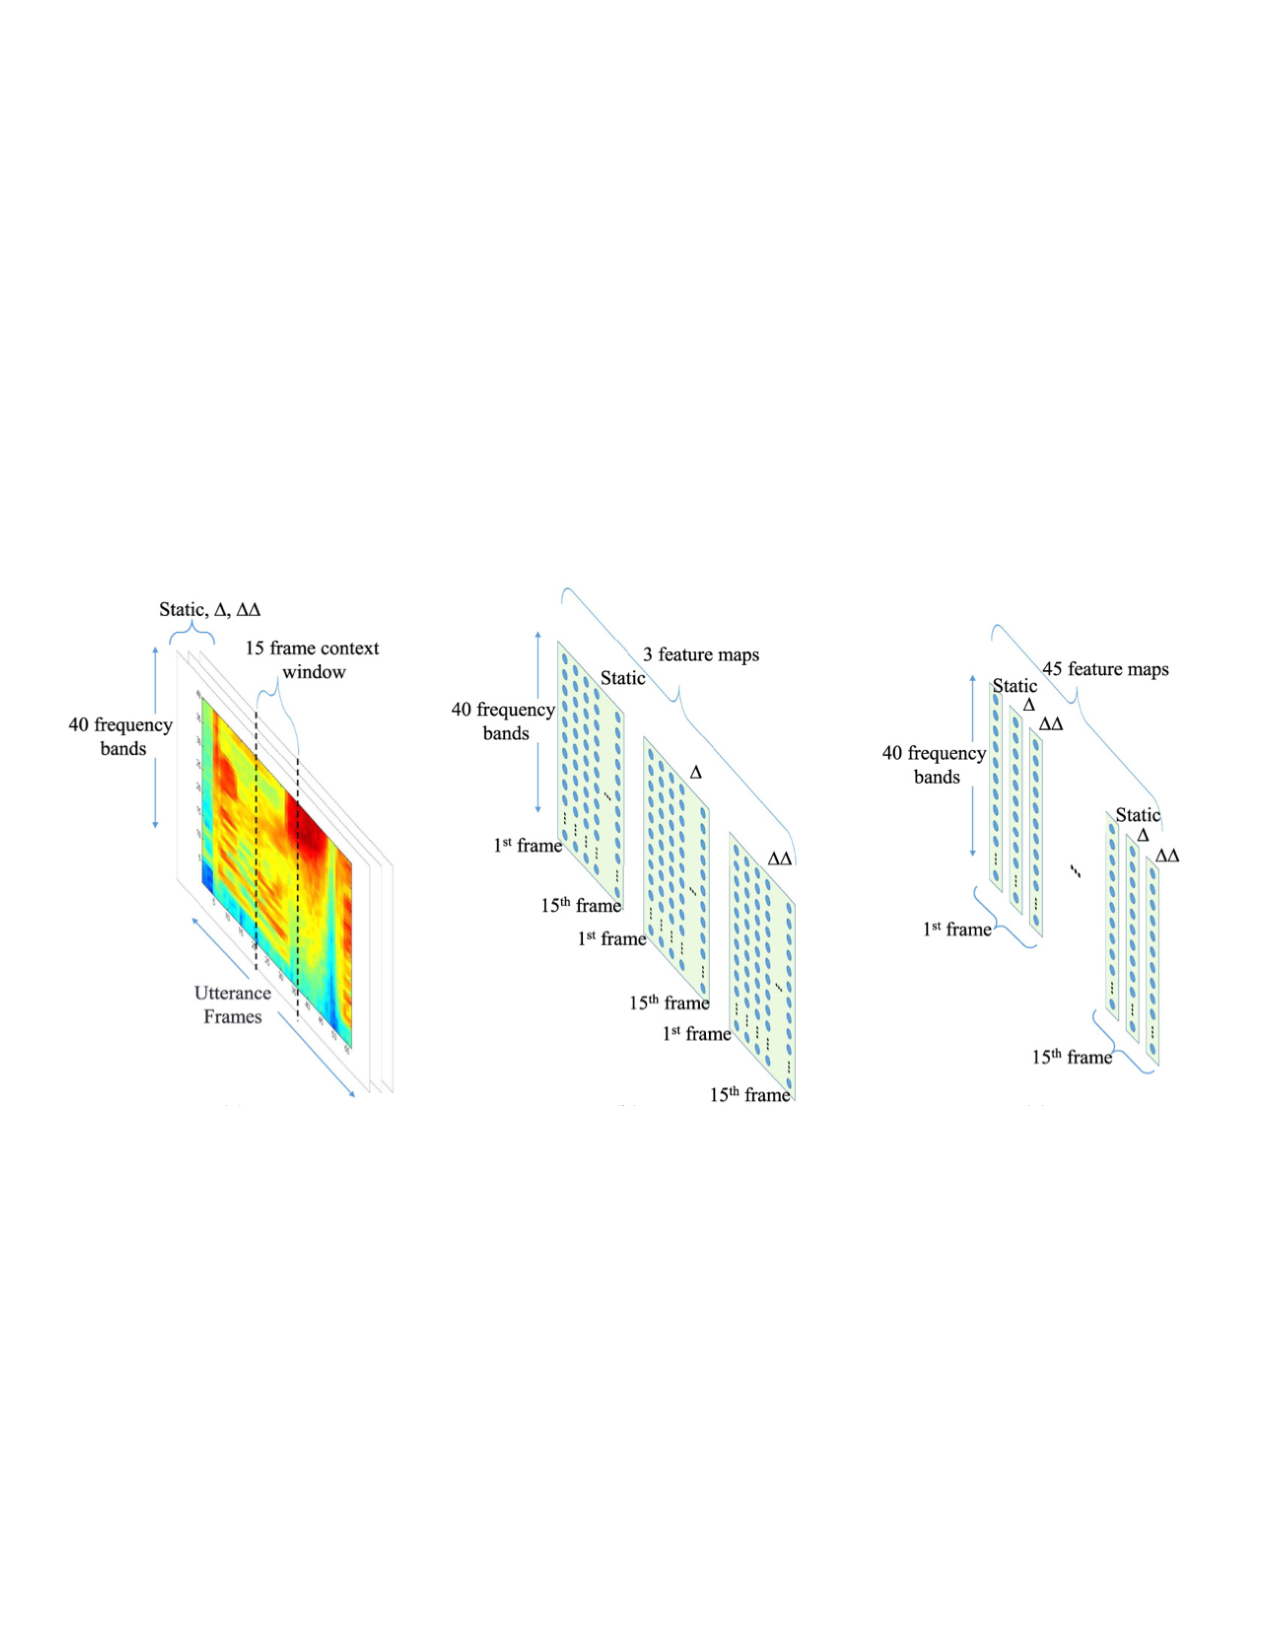
\includegraphics[scale=0.6, trim=1.1cm 0 0 7.5cm, clip=true]{cnn-input.pdf}

\end{frame}

\begin{frame}
	\frametitle{Global Architecture}
	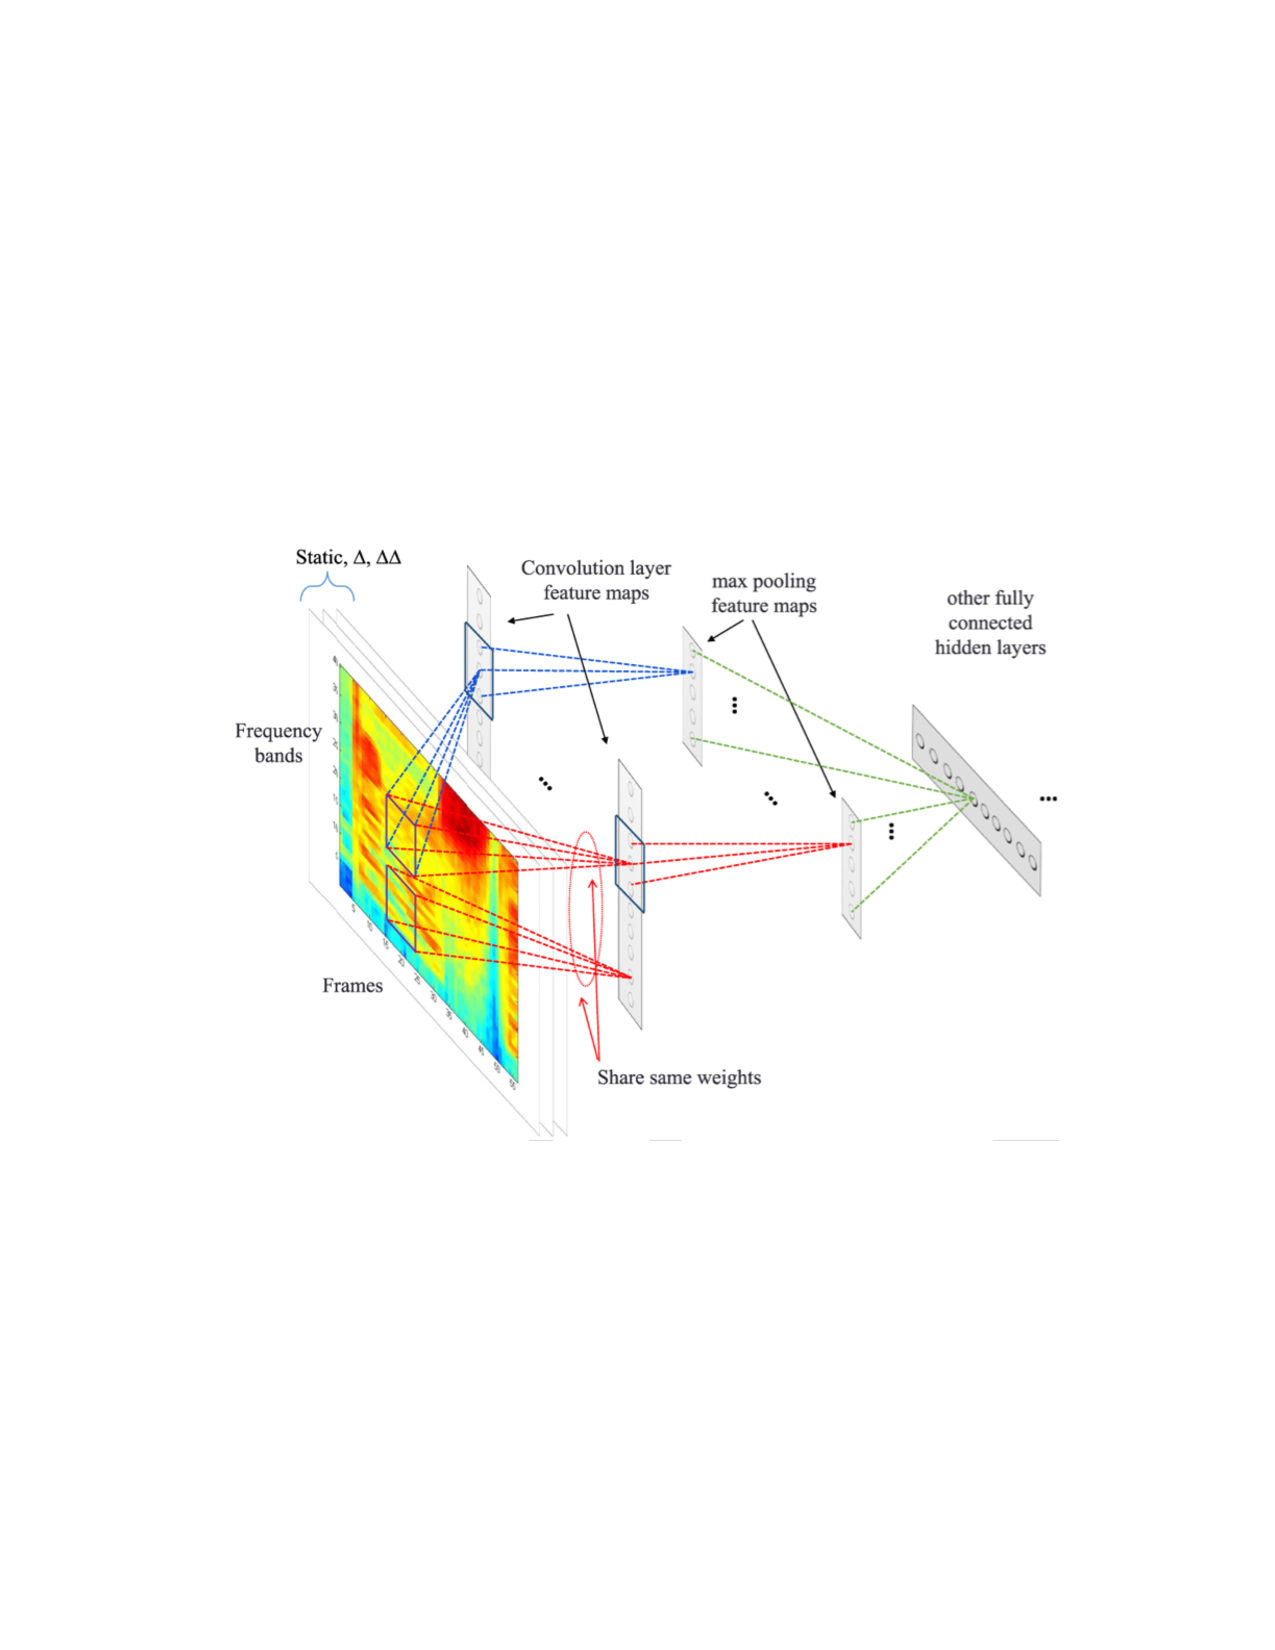
\includegraphics[scale=0.65, trim=2cm 0 0 8cm, clip=true]{cnn-global.pdf}
\end{frame}

\begin{frame}
	\frametitle{Convolution Ply}
	\begin{center}
		The convolution ply introduces locality into the network. Unlike in image processing, weights are only shared between neurons that go to the same pooling ply. 
	\end{center}
	
	\begin{center}
		Limited weight sharing is used to reflect the fact that properties of the speech signal vary over different frequency bands. Each frequency band has its own shared weights.
	\end{center}	
	\vfill
	\begin{center}
		Each unit in a single feature map can be computed as below:
	\end{center}
	\begin{equation*}
	q_{j,m} = \sigma(\sum_{i=1}^{I}\sum_{n=1}^{F}o_{i,n+m-1}w_{i,j,n}+w_{0,j}), (j = 1, ..., J)
	\end{equation*}

\end{frame}

\begin{frame}
	\frametitle{Pooling Ply}
	\begin{center}
		The pooling ply reduces the resolution of the feature maps, serving as a generalization over the features of the convolution ply. This helps with handling small shifts in frequency.
	\end{center}
	\begin{center}
		In this paper they use a simple max-pooling function:
	\end{center}
	\begin{equation*}
	p_{i,m} = \max_{n=1}^{G} q_{i, (m-1)xs+n}
	\end{equation*}
	\begin{center}
		where \textit{G} is the pooling size and \textit{s} is the shift size. If \textit{G = s}, there is no overlap between the pooling windows.
	\end{center}
	
\end{frame}

\begin{frame}
	\frametitle{A Simpler Example}
	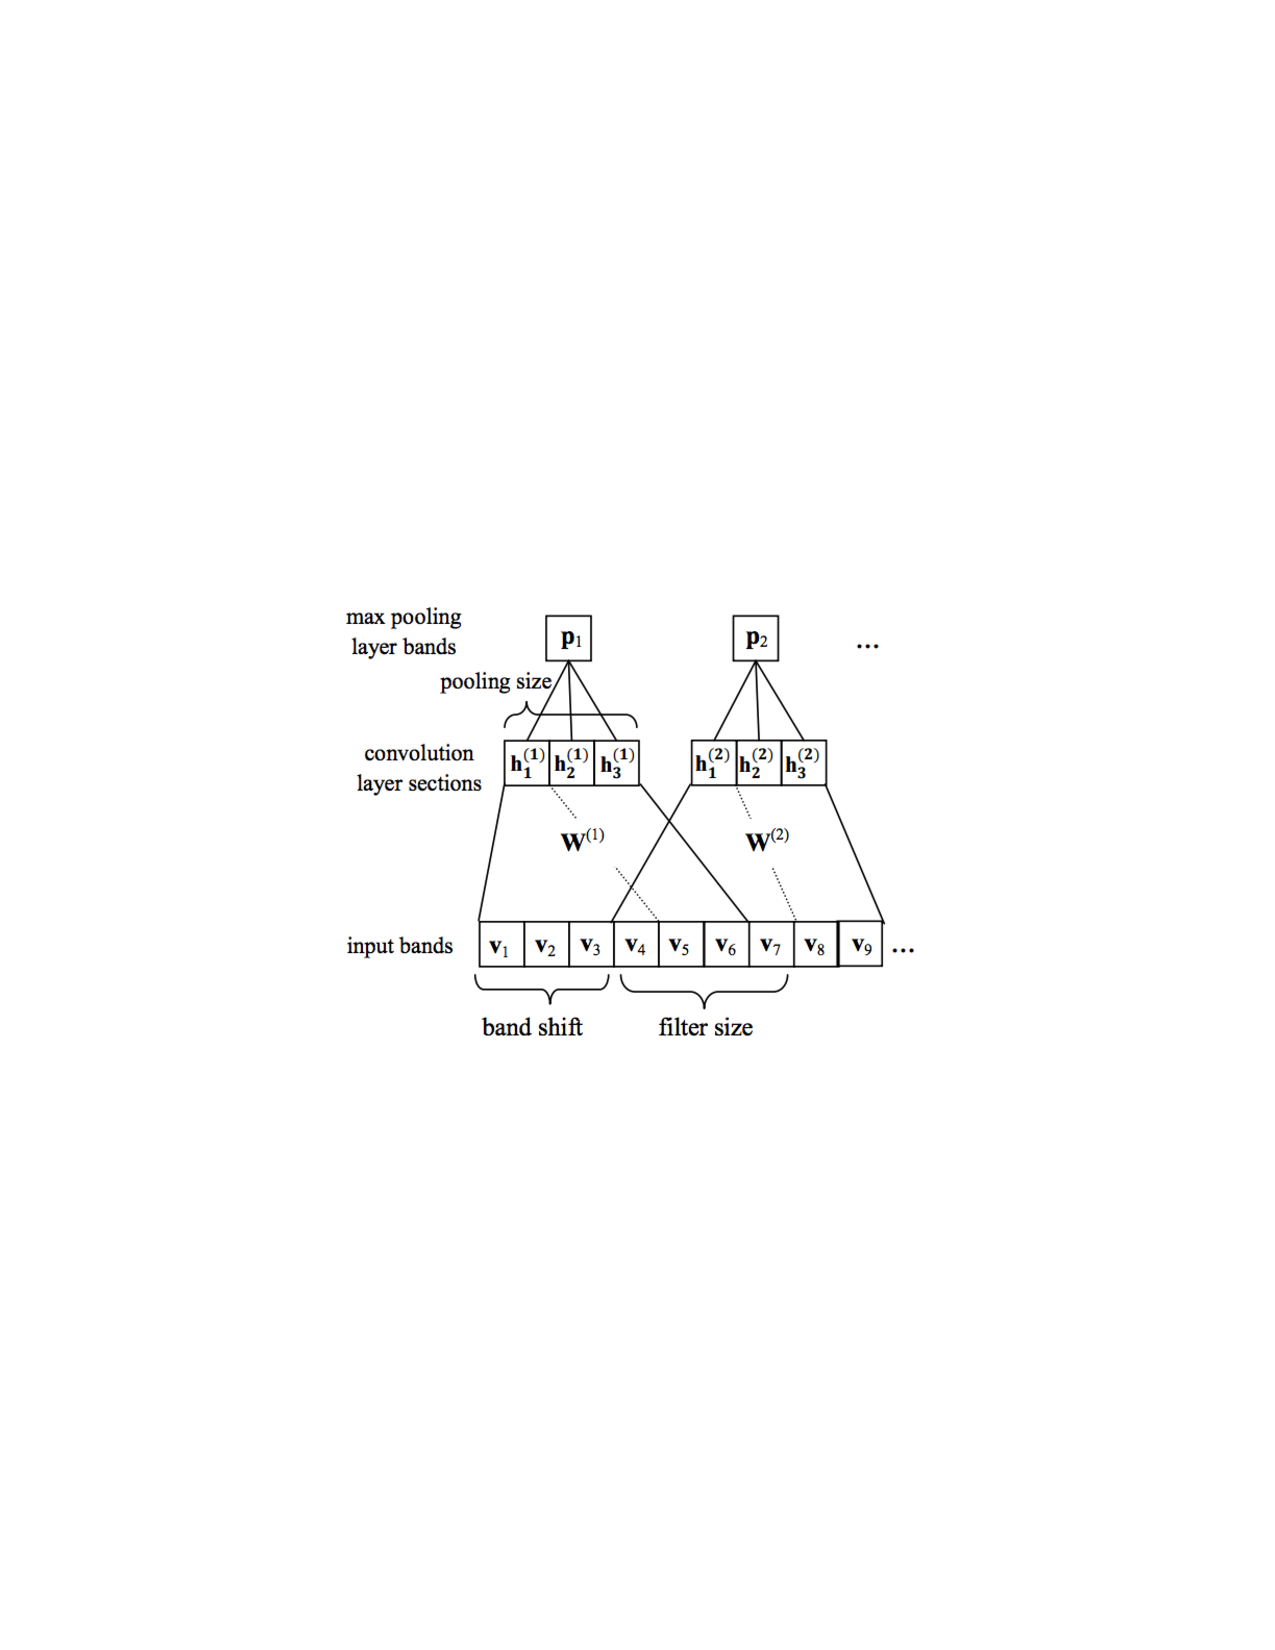
\includegraphics[scale=1, clip=true, trim=5cm 0 0 10cm]{conv-pool.pdf}
\end{frame}

\begin{frame}
	\frametitle{Training with Back-Propagation}
	\begin{center}
		Most frequently used training algorithm for ANNs. We want to discover how the output of the ANN changes with respect to the input. Both networks use a softmax output layer to compute the posterior probability:
		\begin{equation*}
		y_{i} = \frac{\exp(o_{i}^{(L)})}{\sum_{j}\exp(o_{j}^{(L)})}
		\end{equation*}
		Goal is to minimize the cross-entropy function: $Q({W^{(l)}}) = -\sum_{i}d_{i}\log y_{i}$ where \textit{d} is the target and \textit{y} is the prediction.
		\vfill
		Compute derivative of Q with respect to each weight matrix, and use stochastic gradient descent to minimize the objective function.
	\end{center}
\end{frame}

\begin{frame}
	\frametitle{Back-Propagation cont.}
	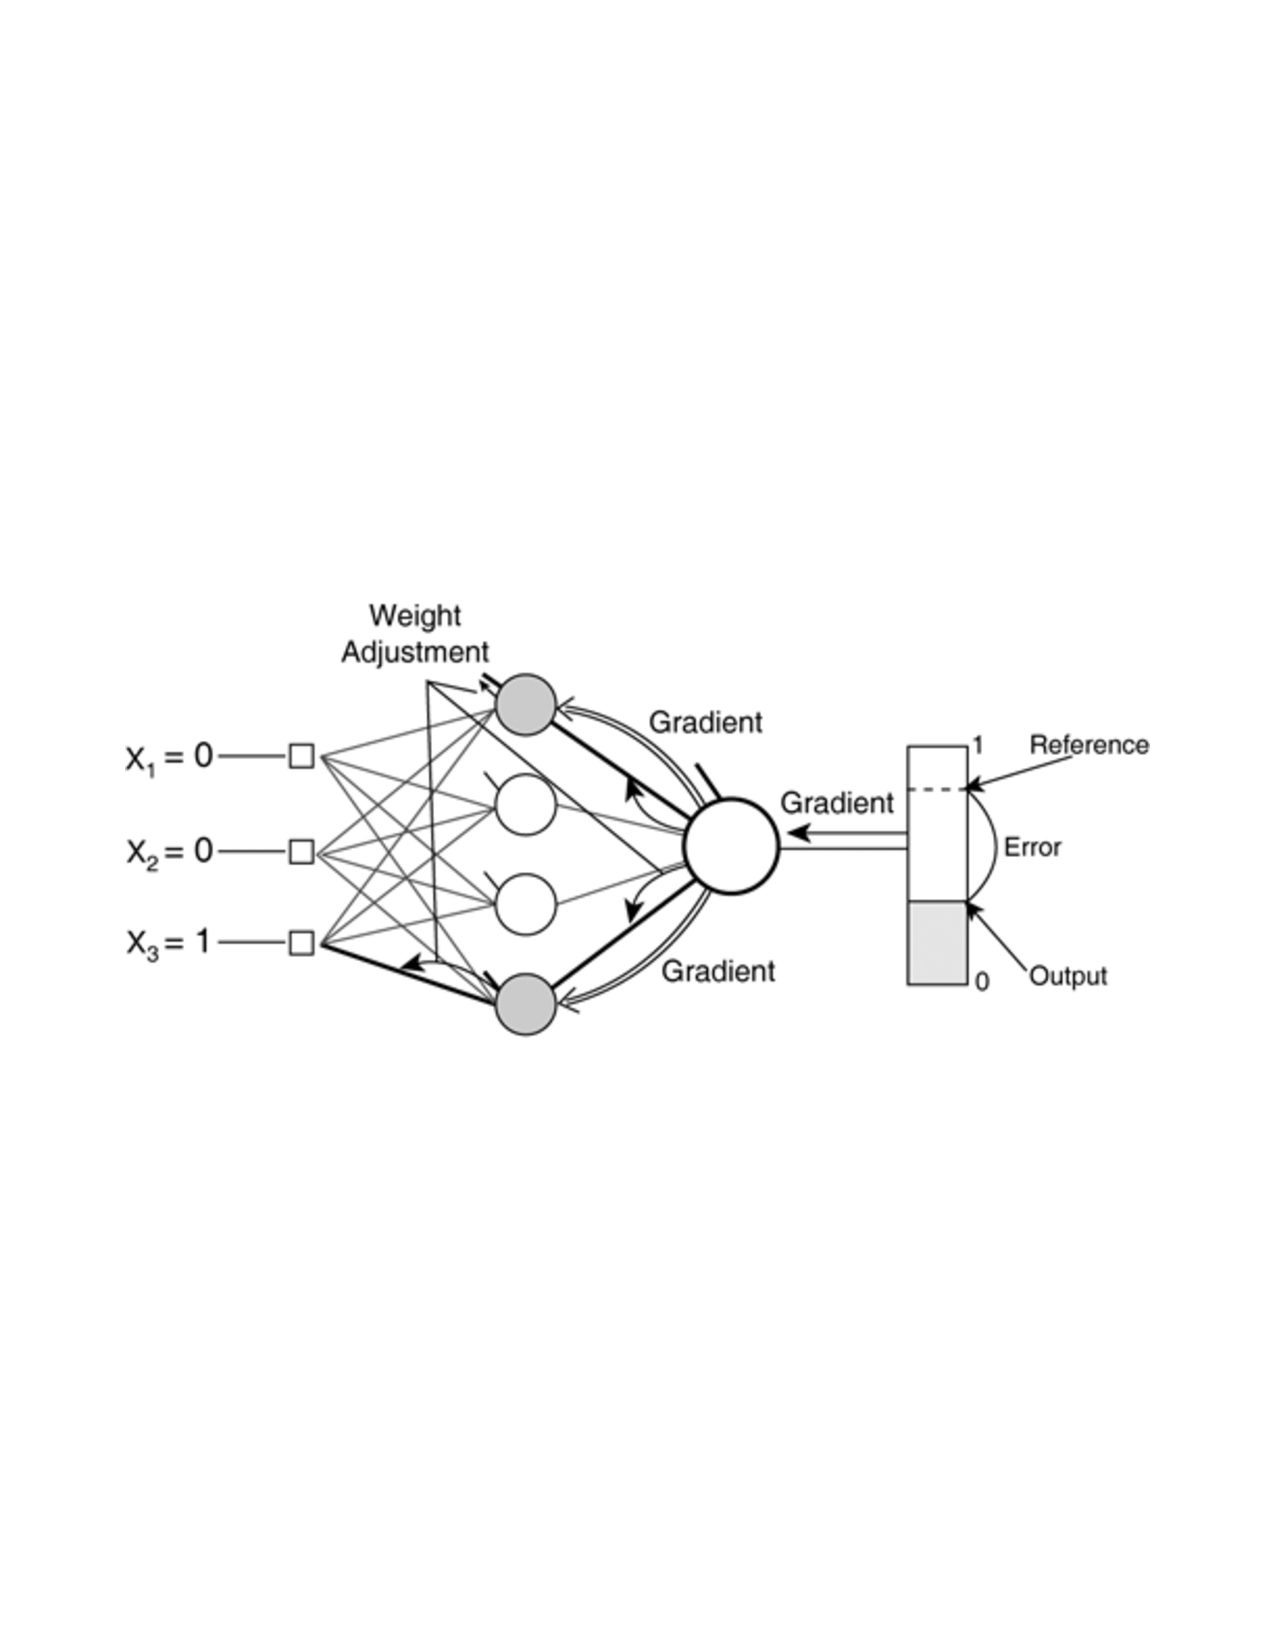
\includegraphics[scale=0.65, trim=2cm 0 0 8cm, clip=true]{backprop.pdf}
\end{frame}

\begin{frame}
	\frametitle{Outline}
	
	\begin{enumerate}
		\item Introduction
		\item Gaussian Mixture Models
		\item Convolutional Neural Networks
		\item \textcolor{blue}{Deep Neural Networks}
		\item Experimental Results
		\item Conclusions
	\end{enumerate}
\end{frame}

\begin{frame}{Deep Neural Networks}
	\begin{center}
	\textbf{Context-Dependent Pre-Trained Deep Neural Networks for Large-Vocabulary Speech Recognition}
	\end{center}
	
	\vfill

	\hfill George Dahl \hfill Dong Yi \hfill Li Deng \hfill Alex Acero \hfill
	
	\vfill
	
	\begin{center}
		IEEE Transactions on Audio, Speech, and Language processing, Vol. 20, No. 1, January 2012
	\end{center}
	
\end{frame}
	
\begin{frame}{Problem Formulation}
	\begin{center}
		Noisy channel model: maximize the likelihood of a decoded word sequence, $\hat{w}$, given our observed audio input, $x$:
	\end{center}
	 
	\vfill
	
	\begin{equation*}
		\hat{w} = \argmax{w \in \mathscr{L}} \underbrace{\cprob{x}{w}}_{\text{ Accoustic Model }} \underbrace{\prob{w}}_{\text{ Language Model }} 
	\end{equation*}
	
	\vfill
	
	\begin{center}
		Use N-gram language model, CD-DNN-HMM for acoustic model
	\end{center}
\end{frame}

\begin{frame}{Problem Formulation (Cont)}
	\begin{center}
	Here the acoustic model is viewed as a sequence of transitions between states of tied-state triphones referred to as \textbf{senones}.
	\end{center}
	
	\vfill
	
	\begin{equation*}
	\underbrace{\cprob{x}{w}}_{\text{ Accoustic Model }} \approxeq \max \underbrace{\pi(q_0)}_{ \text{ Init State } } \prod_{t = 1}^T \underbrace{ a_{q_{t-1} q_t} }_{ \text{ Transistion } } \prod_{t=0}^T \underbrace{ \cprob{x_t}{q_t} }_{ \text{ Senone posterior } } 
	\label{eqn:lm:def}
	\end{equation*}
	
	\vfill
	
	\begin{center}
		Where $\cprob{x_t}{q_t}$ models the tied triphone senone posterior given mel-frequency cepstral coefficients (\textbf{MFCCs}) based on 11 sampled frames of audio.
	\end{center}
\end{frame}
	
\begin{frame}{Deep Neural Networks}
	\resizebox{\linewidth}{!}{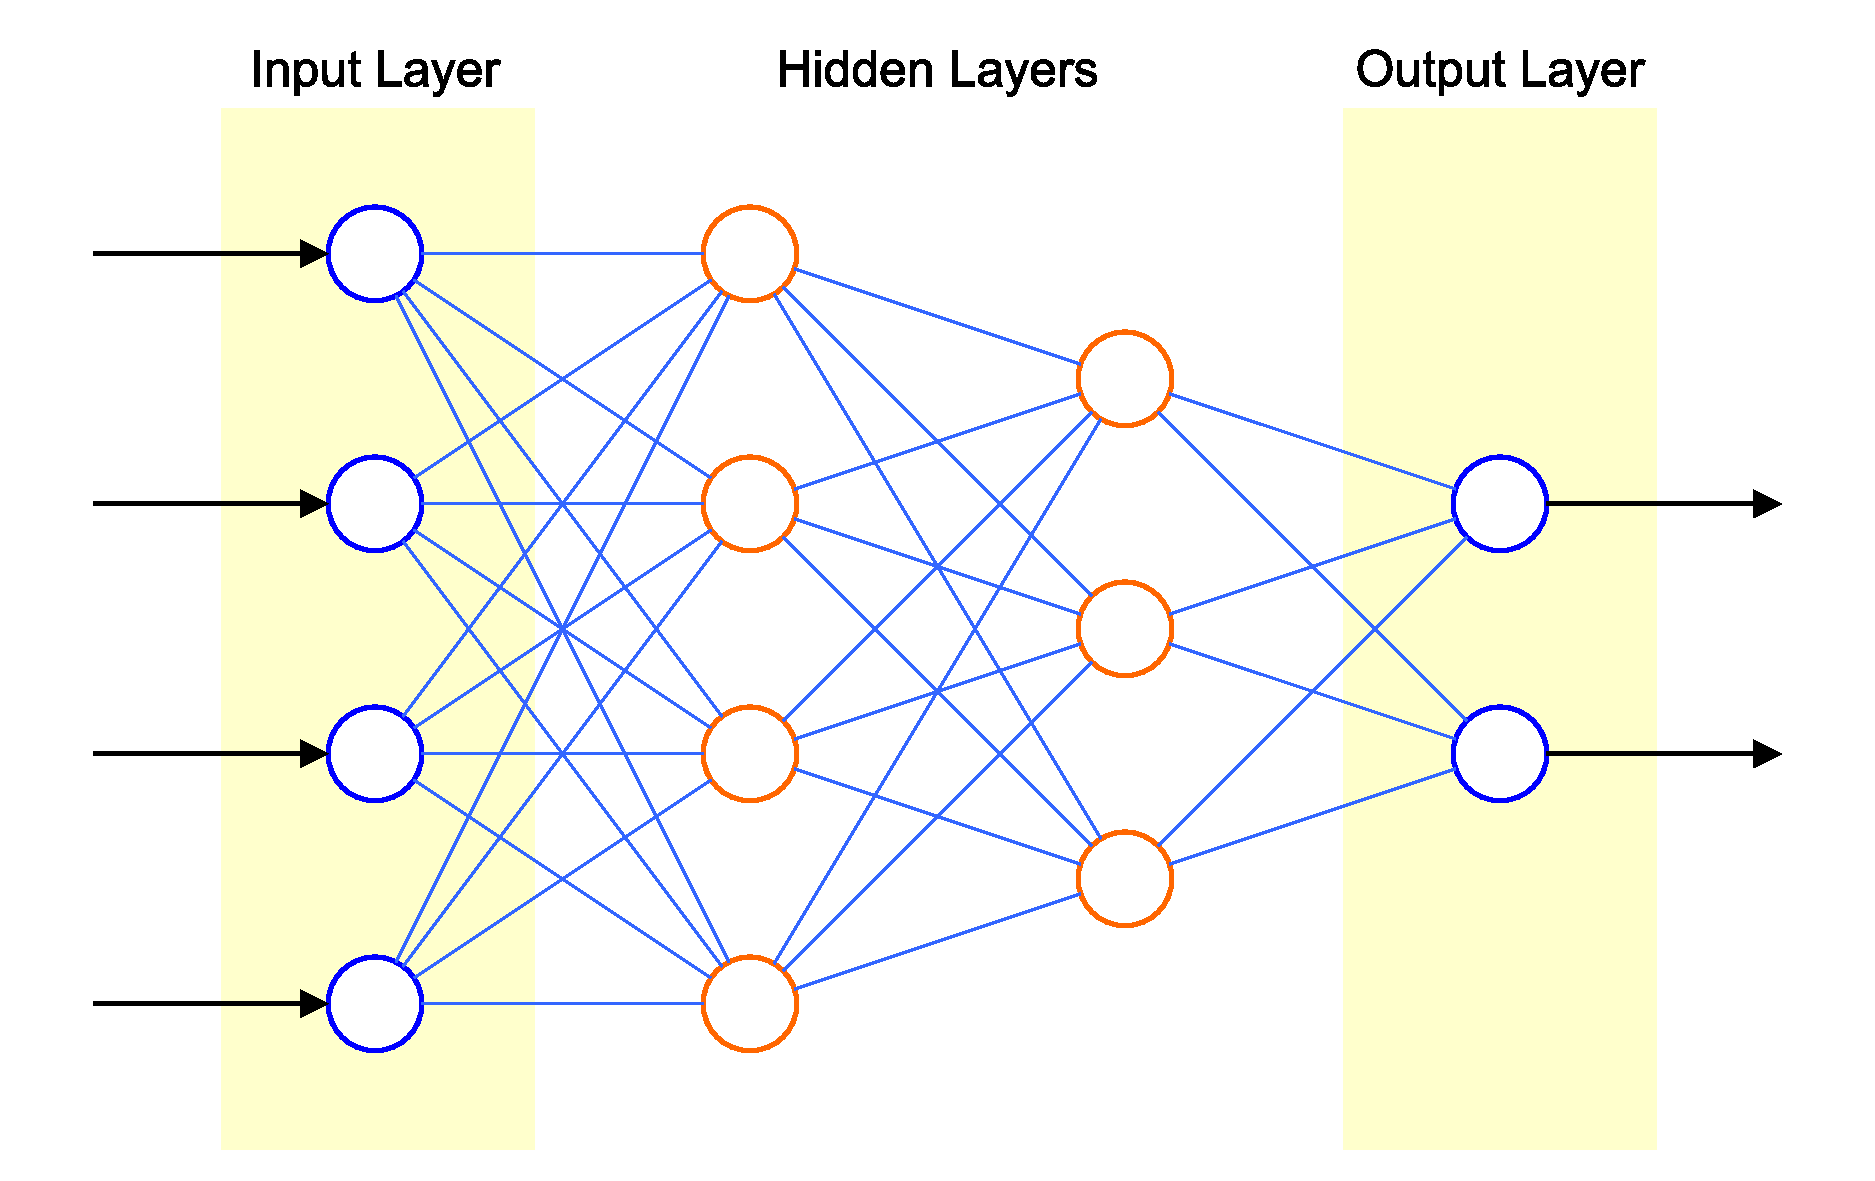
\includegraphics{dnn.pdf}}
\end{frame}

\begin{frame}{Training}
	\begin{center}
		Training is complicated and time intensive! At a very high level two steps: initialization and DNN training.
	\end{center}
	
	\vfill
	
	Initialization:
	\begin{itemize}
		\item Find the best tying of triphone states
		\item Deal with some book keeping
		\item Train a CD-GMM-HMM using those states.
		\item Convert CD-GMM-HMM into CD-DNN-HMM keeping senone structure
		\item Apply pre-training algorithm on CD-DNN-HMM
	\end{itemize}

	\vfill	

\end{frame}

\begin{frame}{Training}

\vfill

DNN Training:

\begin{itemize}
	\item Generate raw alignment of states to senones
	\item Use alignment to refine by backpropagation
	\item Re-estimate prior senone probability given frames
	\item Refine HMM transitions probabilities
	\item Goto first step if no improvement against development set
\end{itemize}

\vfill

\vfill

\begin{center}
Just enough time to talk about one of these steps in detail. Let's look at pre-training...
\end{center}

\vfill


\end{frame}


\begin{frame}{Pre-Training In-Depth}
	\vfill

	\begin{center}
		DNN training computationally intractable until Hinton et al. come to the rescue with \textit{A Fast Learning Algorithm for Deep Belief Nets}.
	\end{center}
	
	\vfill

	\begin{center}
		Big idea: Use an approximate method, \textbf{contrastive divergence}, to get near an optimal solution, then use traditional methods, \textbf{backpropagation}, to finish the job. 
	\end{center}
	
	\vfill
	
	\begin{center}
		Need to understand Restricted Boltzmann Machines (RBMs) and Deep Belief Networks (DBNs)
	\end{center}
	
	\vfill
\end{frame}

\begin{frame}{Pre-Training: RBMs and DBNs}
	\vfill

	\begin{columns}
		\begin{column}{0.4\linewidth}
			\begin{center}
				Bipartite arrangement of weights is assigned an energy:
			\end{center}
		
			\begin{equation*}	
				E(v, h) = - b^T v - c^T h - v^T W h
			\end{equation*}
		\end{column}
		\begin{column}{0.6\linewidth}
			\resizebox{\linewidth}{!}{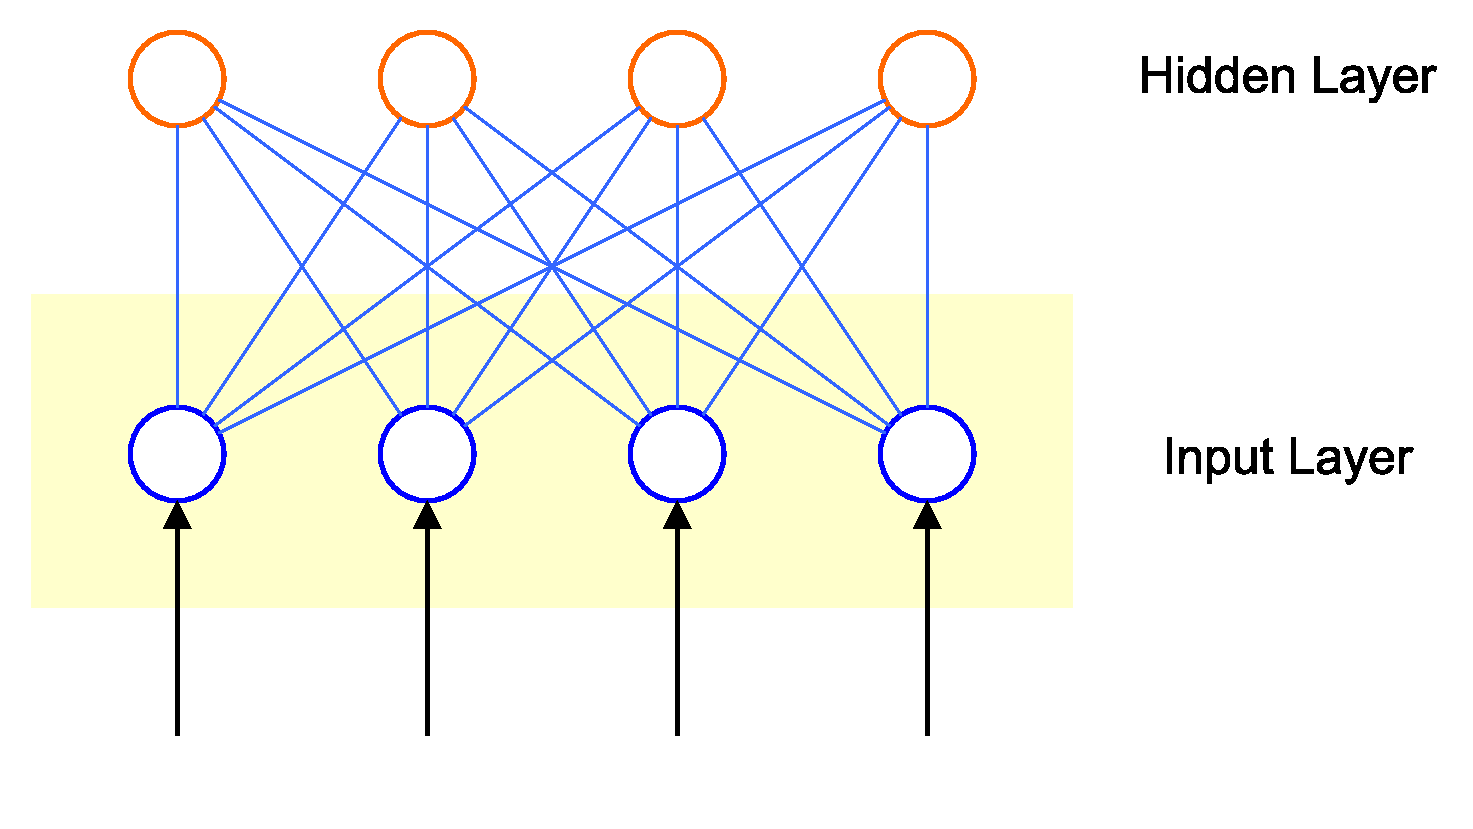
\includegraphics{rbm.pdf}}
		\end{column}
	\end{columns}
	
	\vfill

	\begin{center}
		For purpose of this talk, stack RBMs on top of one another to get a DBN
	\end{center}

	\vfill
\end{frame}

\begin{frame}{Pre-Training: Contrastive Divergence}
		\begin{center}
			Want to do vanilla Stochastic Gradient Descent, however, our \textcolor{blue}{model} term takes \textbf{exponential} time to compute correctly. 
		\end{center}
		
		\begin{equation*}
			- \partialDx{\ell(\theta)}{w_{ij}} = \inAngle{ \partialDx{E}{\theta} }_\text{data} - \inAngle{ \partialDx{E}{\theta} }_\text{\textcolor{blue}{model}}
		\end{equation*}
		
		\begin{center}
			Instead, \textbf{approximate} it (essentially minimizing Kullback-Leibler divergence) with \textcolor{blue}{one step} Gibbs sampling:
		\end{center}
		
		\begin{equation*}
			- \partialDx{\ell(\theta)}{w_{ij}} \approx \inAngle{ v_i h_j }_\text{data} - \inAngle{ v_i h_j }_\text{\textcolor{blue}{1}}
		\end{equation*}
\end{frame}

\begin{frame}{Pre-Training: Bringing it all together}
	\begin{columns}
		\begin{column}{0.45\linewidth}
			Hinton's Greedy Algorithm:
		
			\hfill
		
			1) Train RBM consisting of first two layers
			
			\hfill
			
			2) Move RBM frame up a layer and train

			\hfill 
			
			3) When out of layers, you have trained DBN
			
			\hfill
			
			4) Refine with backpropagation
		\end{column}
		\begin{column}{0.55\linewidth}
			\resizebox{\linewidth}{!}{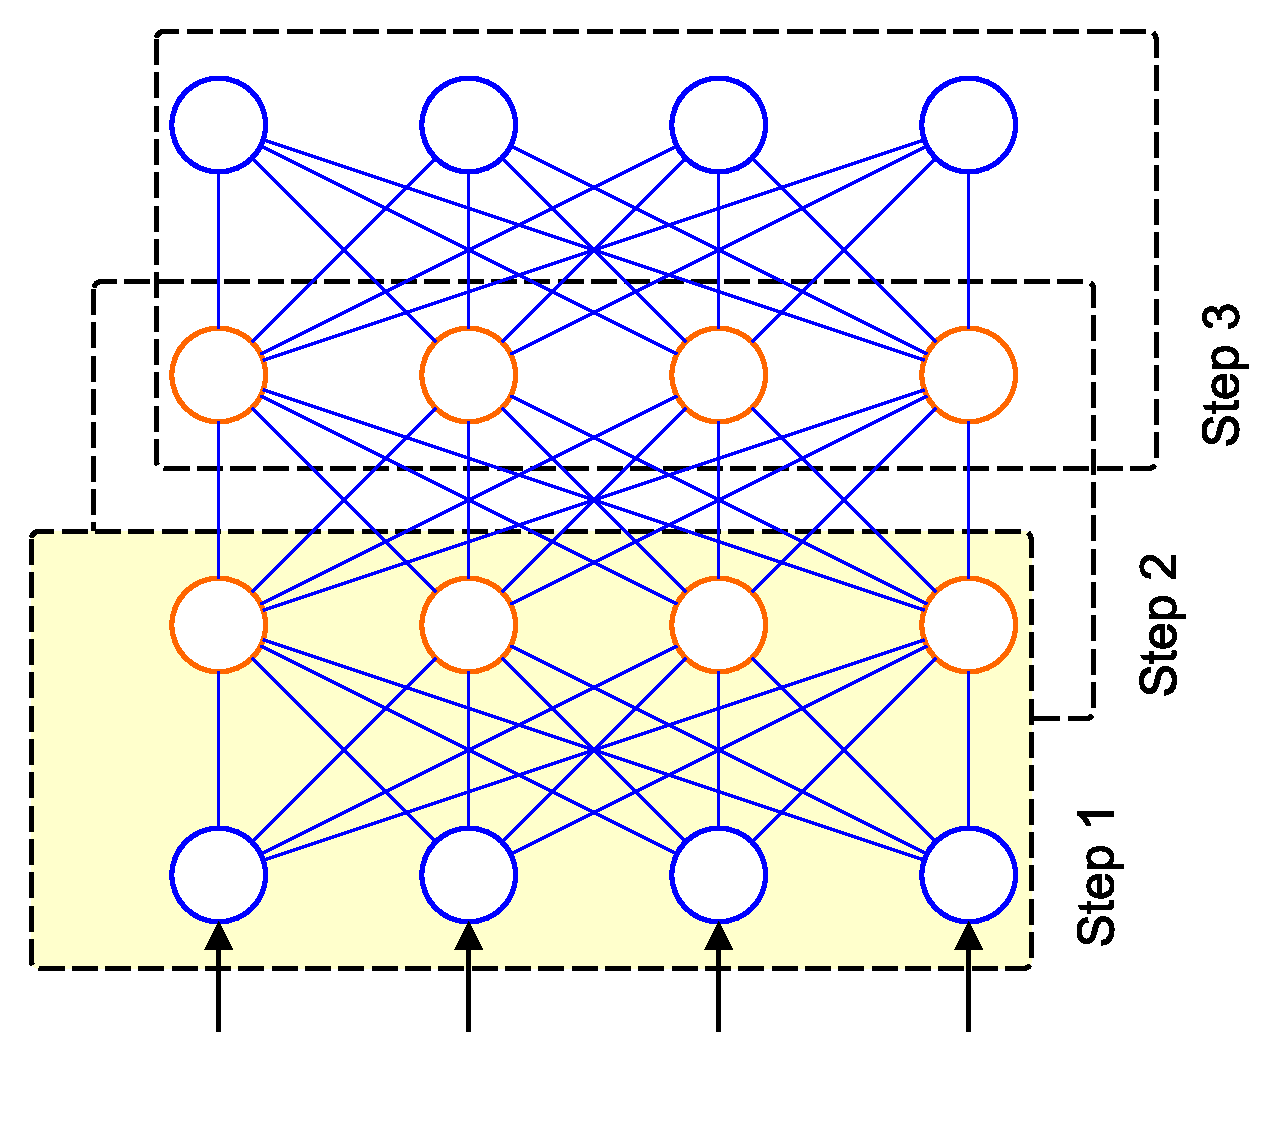
\includegraphics{dbn.pdf}}
		\end{column}
	\end{columns}

\end{frame}

\begin{frame}
	\frametitle{Outline}
	
	\begin{enumerate}
		\item Introduction
		\item Gaussian Mixture Models
		\item Convolutional Neural Networks
		\item Deep Neural Networks
		\item \textcolor{blue}{Experimental Results}
		\item Conclusions
	\end{enumerate}
\end{frame}

\begin{frame}{Experimental Results}

\begin{table}[H]
	\begin{center}
		Papers report different metrics (sentence accuracy, phone error rate) on different datasets (Bing, TIMIT) 
	\end{center}
	
	\vfill

	\centering
	\begin{tabular}{c|c|c|c|c}
		& \multicolumn{2}{c|}{Bing Mobile} & \multicolumn{2}{c}{TIMIT}\\
		Architecture & Dev. & Test  & Dev. & Test \\
		\hline
		CD-GMM-HMMM & 70.3\% & 68.4\% & & \\
		CD-DNN-HMM & 71.8\% & 69.6\% & & \\
		\hline
		CNN-HMM  & & &  & 20.07\%
	\end{tabular}

	\vfill

	\begin{center}
		Take away: Both demonstrate significant improvement over GMM approach, with CNN approach giving the best performance.
	\end{center}
\end{table}

\end{frame}

\begin{frame}
	\frametitle{Outline}
	
	\begin{enumerate}
		\item Introduction
		\item Gaussian Mixture Models
		\item Convolutional Neural Networks
		\item Deep Neural Networks
		\item Experimental Results
		\item \textcolor{blue}{Conclusions}
	\end{enumerate}
\end{frame}

\begin{frame}{Conclusions}
	\TODO{Garrett}
\end{frame}

\begin{frame}{Conclusions (Cont)}
	\TODO{Garrett}
\end{frame}

\begin{frame}
	\begin{center}
		Questions?
	\end{center}
\end{frame}

\end{document}
